\section*{1\quad Introduction}

Let $(Z_0,Z_1,\ldots)$ be a \emph{Galton-Watson branching process with offspring distribution} $(p_i;\ i=0,1,\ldots)$, where $p_i\ge 0$, $\sum_i p_i=1$. Interpret $p_i$ as the probability that an individual has $i$ children, and $Z_g$ as the number of individuals in the $g$th generation of a population starting from some initial number $Z_0$. For each $g\ge 0$, it is assumed that given the evolution of the population up to the $g$th generation, the $Z_g$ individuals in the $g$th generation have independent random numbers of children distributed according to $(p_i)$. These children are the $Z_g$ members of the $(g+1)$th generation. See [30, 33, 5] for background.

Let
\[
S_n:=X_1+\cdots+X_n \tag{1}
\]
be the sum of $n$ independent random variables $X_j$ with common distribution $(p_i)$. From the description of $(Z_0,Z_1,\ldots)$, this sequence is a Markov chain with state space $\{0,1,2,\ldots\}$ and time-homogeneous transition probabilities
\[
P(Z_{g+1}=m\mid Z_g=n)=P(S_n=m) \tag{2}
\]
where for each $n$ the sequence $(P(S_n=m),\ m=0,1,\ldots)$ is the $n$-fold convolution of the sequence $(p_i;\ i=0,1,\ldots)$ with itself. Two elementary expressions for $P(S_n=m)$ in terms of $(p_i)$ are recalled in formulae (7) and (8) below. Let
\[
\#\mathcal{F}_k:=\sum_{g=0}^{\infty} Z_g\in\{1,2,\ldots,\infty\} \tag{3}
\]
represent the \emph{total progeny} in the branching process given $Z_0=k$ individuals to start with. Here $\#\mathcal{F}_k$ stands for the number of individuals in the random family $\mathcal{F}_k$ generated by the branching process. In Section 4, $\mathcal{F}_k$ will be defined as a \emph{random family forest}, that is a collection of $k$ \emph{random family trees}, one for each of the $k$ initial individuals. The following theorem presents a remarkable formula for the distribution of $\#\mathcal{F}_k$ restricted to positive integers. This formula was discovered by Otter [43] for $k=1$ and extended to all $k\ge 1$ by Dwass [17]:

\textbf{Theorem 1} (Otter-Dwass formula) \emph{For all $n,k=1,2,\ldots$}
\[
P(\#\mathcal{F}_k=n)=\frac{k}{n}P(S_n=n-k). \tag{4}
\]

The first approach to these formulae was by the method of probability generating functions. Let
\[
g(z):=\sum_{i=0}^{\infty} p_i z^i \tag{6}
\]
be the probability generating function derived from the offspring distribution $(p_i)$. Two elementary expressions for $P(S_n=m)$ are
\begin{align}
P(S_n=m)&=\text{coefficient of } z^m \text{ in } g(z)^n \tag{7}\\
&=\sum_{\substack{\Sigma n_i=n\\ \Sigma i n_i=m}} \binom{n}{n_0,\ldots,n_n}\prod_{i\ge 0} p_i^{n_i} \tag{8}
\end{align}
where the sum ranges over the finite set of all sequences of non-negative integers $(n_i,i\ge 0)$ with $\Sigma n_i=n$ and $\Sigma i n_i=m$. Here
\[
\binom{n}{n_0,\ldots,n_n}:=\frac{n!}{n_0!\cdots n_n!} \tag{9}
\]
is the multinomial coefficient which is the number of sequences $(i_j,1\le j\le n)$ of \emph{type} $(n_i,i\ge 0)$, that is sequences $(i_j)$ such that $\#\{j: i_j=i\}=n_i$ for all $i\ge 0$ and hence $\sum_j i_j=\sum_i i n_i$.

The term \emph{forest} will be used here for a \emph{finite rooted forest}, that is a directed graph with a finite number of vertices, each of whose connected components is a tree with edges directed away from its root vertex. A forest with vertex set $V$ is said to be \emph{labeled by $V$}. For vertices $v$ and $w$ of a forest $\mathbf{f}$ write $v\xrightarrow{\mathbf{f}} w$ to show that $(v,w)$ is a directed edge of $\mathbf{f}$. The \emph{number of children} or \emph{out-degree} $v$ in the forest $\mathbf{f}$ is $C(v,\mathbf{f}):=\#\{w: v\xrightarrow{\mathbf{f}} w\}$. In a \emph{plane forest} $\mathbf{f}$ with $k$ component trees, the set of roots of the tree components is ordered, as is the set of children of $v$ for each vertex $v$ of $\mathbf{f}$. Regard a plane forest with $k$ root vertices as a collection of family trees, one for each of $k$ initial individuals, with each vertex in the forest corresponding to an individual, and with the order of the roots and the orders of children corresponding to the order of birth of individuals. A plane forest is often depicted without labels as on the left side of Figure 1, and called an \emph{unlabeled plane forest}. However, there is a natural way to identify each vertex of a plane forest by a finite sequence of non-negative integers which indicates the location of the vertex in the forest. So, following the convention of [30] for labeling family trees, the set of vertices of a plane forest will be identified as a subset of the set of all finite sequences of integers, as illustrated on the right side of Figure 1.

\begin{center}
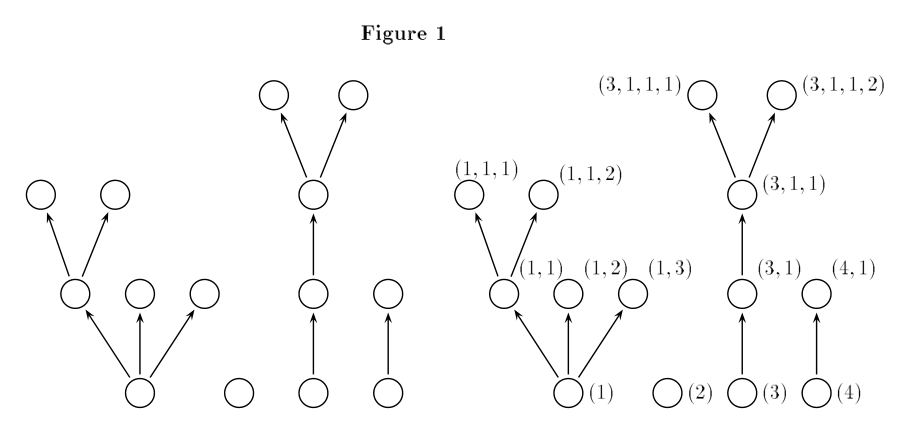
\includegraphics[width=\linewidth]{figures/pitman-tr482-figure-1.png}
\end{center}

An individual in the $g$th generation of a family forest (= vertex at height $g$ in the plane forest) is identified by a sequence of $g+1$ integers, for instance $(3,7,4)$ to indicate a second generation individual who is the 4th child of the 7th child of the 3rd root individual.

The \emph{type} of a forest $\mathbf{f}$ is the sequence of non-negative integers $(n_i)$, where $n_i$ is the number of vertices of $\mathbf{f}$ with $i$ children. Let $1\le k\le n$ and let $(n_i)$ be a sequence of non-negative integers with
\[
\sum_i n_i=n\quad\text{and}\quad \sum_i i n_i=n-k. \tag{12}
\]
A forest of type $(n_i)$ has $n$ vertices and $n-k$ non-root vertices, hence $k$ root vertices and $k$ tree components.

\textbf{Theorem 4} (Enumeration of plane forests by type) [18, 19, 43, 54] \emph{For $1\le k\le n$ and $(n_i)$ subject to (12) the number $N^{\mathit{plane}}(n_0,n_1,\ldots)$ of plane forests of type $(n_i)$ with $k$ tree components and $n$ vertices is}
\[
N^{\mathit{plane}}(n_0,n_1,\ldots)=\frac{k}{n}\binom{n}{n_0,\ldots,n_n}. \tag{13}
\]

\textbf{Theorem 5} (Enumeration of labeled forests by type) [59, Cor.\ 3.5] \emph{Let $[n]:=\{1,\ldots,n\}$. For $1\le k\le n$ and $(n_i)$ subject to (12), the number $N^{[n]}(n_0,n_1,\ldots)$ of forests labeled by $[n]$ of type $(n_i)$ with $k$ tree components and $n$ vertices is}
\[
N^{[n]}(n_0,n_1,\ldots)=\frac{k}{n}\binom{n}{k}\frac{(n-k)!}{\prod_{i\ge 0}(i!)^{n_i}}\binom{n}{n_0,\ldots,n_n}. \tag{14}
\]

The enumeration of plane forests by type is simpler than its companion for labeled forests. But the result for labeled forests has the following simpler equivalent:

\textbf{Theorem 6} (Enumeration of labeled forests by out-degree sequence) [51],[59, Thm.\ 3.4] \emph{For all sequences of non-negative integers $(c_1,\ldots,c_n)$ with $\sum_i c_i=n-k$ the number $N(c_1,\ldots,c_n)$ of forests $\mathbf{f}$ with vertex set $[n]$ in which vertex $i$ has $c_i$ children for each $i\in[n]$ (and hence $\mathbf{f}$ has $k$ tree components) is}
\[
N(c_1,\ldots,c_n)=\frac{k}{n}\binom{n}{k}\binom{n-k}{c_1,\ldots,c_n}. \tag{15}
\]
